\chapter{Appendix}
\label{app}

\section{Geometric Programming}
\label{a:gpintro}

Introduced in 1967 by Duffin et al.~\cite{duffingp}, a geometric program \gls{GP} is
a type of constrained optimization problem that becomes convex after a
logarithmic change of variables. Modern interior point methods allow a typical
sparse \gls{GP} with tens of thousands of decision variables and tens of thousands of
constraints to be solved in minutes on a desktop computer~\cite{convex}. These
solvers do not require an initial guess, and guarantee convergence to a
\textit{global} optimum, assuming a feasible solution exists. If a feasible
solution does not exist, the solver will return a certificate of infeasibility.
These impressive properties are possible because a GP's objective and
constraints consist of only monomial and posynomial functions, which can be
transformed into convex functions in log space.

A monomial is a function of the form
\begin{equation}\label{e:monomial}
m(\mathbf{u}) = c\prod_{j=1}^{n} u_{j}^{a_{j}}
\end{equation}
where $a_{j} \in \mathbb{R}, c \in \mathbb{R}_{++}$ and $u_{j} \in
\mathbb{R_{++}}$. An example of a monomial is the common expression for lift,
$\frac{1}{2} \rho V^2C_{L}S$. In this case, $\mathbf{u} = (\rho, V, C_{L}, S)$,
$c= 1/2$, and $a = (1, 2, 1, 1)$.

A posynomial is a function of the form
\begin{equation}\label{e:posynomial}
p(\mathbf{u}) = \sum_{k=1}^{K}c_{k}\prod_{j=1}^{n} u_{j}^{a_{jk}}
\end{equation}
where $a_{jk} \in \mathbb{R}, c_{k} \in \mathbb{R}_{++}$ and $u_{j} \in
\mathbb{R_{++}}$. A posynomial is a sum of monomials. Therefore, all monomials
are also one-term posynomials.

A GP minimizes a posynomial objective function subject to monomial equality and
posynomial inequality constraints. A GP written in standard form is

\begin{equation}
\label{e:standardform}
\begin{aligned}
\text{minimize }p_{0}(\mathbf{u})& \\
\text{subject to }p_{i}(\mathbf{u})& \leq 1, i = 1, ...., n_{p}, \\
m_{i}(\mathbf{u})& = 1, i = 1, ..., n_{m}
\end{aligned}
\end{equation}

where $p_{i}$ are posynomial functions, $m_{i}$ are monomial functions, and
$\mathbf{u} \in \mathbb{R}^n_{++}$ are the decision variables. Once a problem
has been formulated in the standard form (Equation \ref{e:standardform}), it can
be solved efficiently.

\section{Signomial Programming}
\label{a:spintro}
It is not always possible to formulate a design problem as a GP. This motivates
the introduction of signomials. Signomials have the same form as posynomials
\begin{equation}\label{e:signomial}
s(\mathbf{u}) = \sum_{k=1}^{K}c_{k}\prod_{j=1}^{n} u_{j}^{a_{jk}}
\end{equation}

but the coefficients, $c_{k} \in \mathbb{R}$, can now be any (including
non-positive) real numbers.

A signomial program (SP) is a generalization of GP where the inequality
constraints can be composed of signomial constraints of the form $s(u) \leq 0$..
The log transform of an SP is not a convex optimization problem, but is a
difference of convex optimization problem that can be written in log-space as

\begin{equation}
\begin{aligned}
\text{minimize }f_{0}(\mathbf{x})& \\
\text{subject to }f_{i}(\mathbf{x}) -  g_{i}(\mathbf{x})& \leq 0, i = 1, ...., m
\\
\end{aligned}
\end{equation}

where $f_{i}$ and $g_{i}$ are convex.

There are multiple algorithms that reliably solve signomial programs to
\textit{local} optima~\cite{gpintro, spsolutions}. A common solution heuristic,
referred to as difference of convex programming or the convex-concave procedure,
involves solving a sequence of GPs, where each GP is a local approximation to
the SP, until convergence occurs. It is worth noting that the introduction of
even a single signomial constraint to any GP turns the GP into a \gls{SP}, thus losing
the guarantee of solution convergence to a global optimum. Despite the
possibility of convergence to a local, not global, optimum, SPs are a powerful
tool. The convex approximation, $\hat{f}(x)$, to the non-convex signomial in
log-space, $f(x) - g(x)$, is constructed such that it always satisfies

\begin{equation}
\hat{f}(x) \geq f(x) - g(x) \quad \forall \quad x
\end{equation}

In other words, for each constraint, the feasible set of the convex
approximation $\hat{f}(x) \leq 0$ is a subset of the original SP's feasible set,
$f(x) - g(x) \leq 0$. This means SP inequalities do not require a trust region,
removing the need for trust region parameter tuning and making solving SPs
substantially more reliable than solving general nonlinear programs. Figure
\ref{f:GPapproxs}, where a series of convex (GP compatible) constraints
approximates a non-convex parabolic drag polar in log space, illustrates this
property.

\begin{figure*}[t!]
    \centering
    \begin{subfigure}[t]{0.5\linewidth}
        \centering
        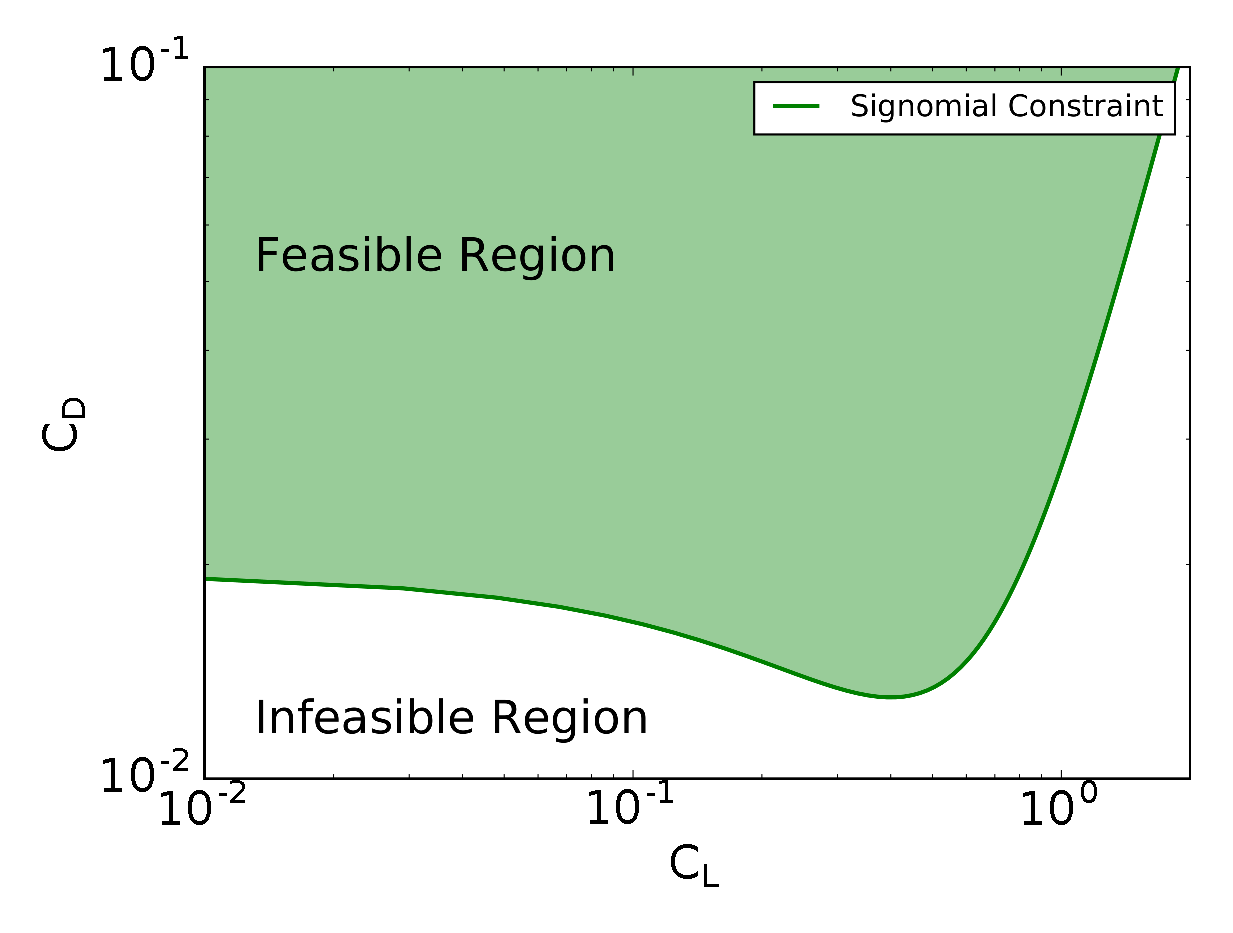
\includegraphics[width=0.9\linewidth]{posyapprox0.eps}
        \caption{Non-convex signomial inequality drag constraint}
    \end{subfigure}%
    ~
    \begin{subfigure}[t]{0.5\linewidth}
        \centering
        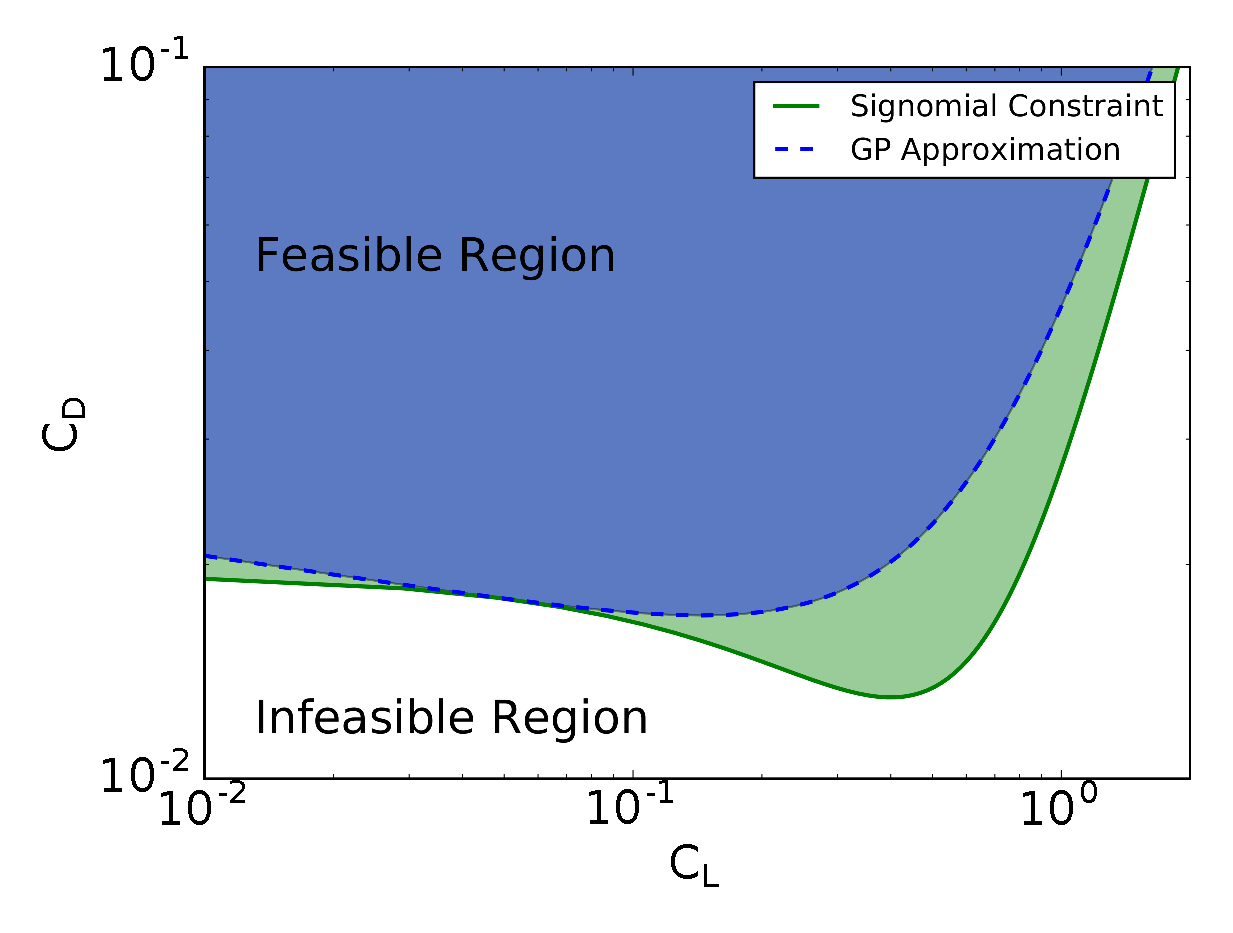
\includegraphics[width=0.9\linewidth]{posyapprox1.eps}
        \caption{Convex approximation about $C_{L} = 0.05$.}
    \end{subfigure}
    \begin{subfigure}[b]{0.5\linewidth}
        \centering
        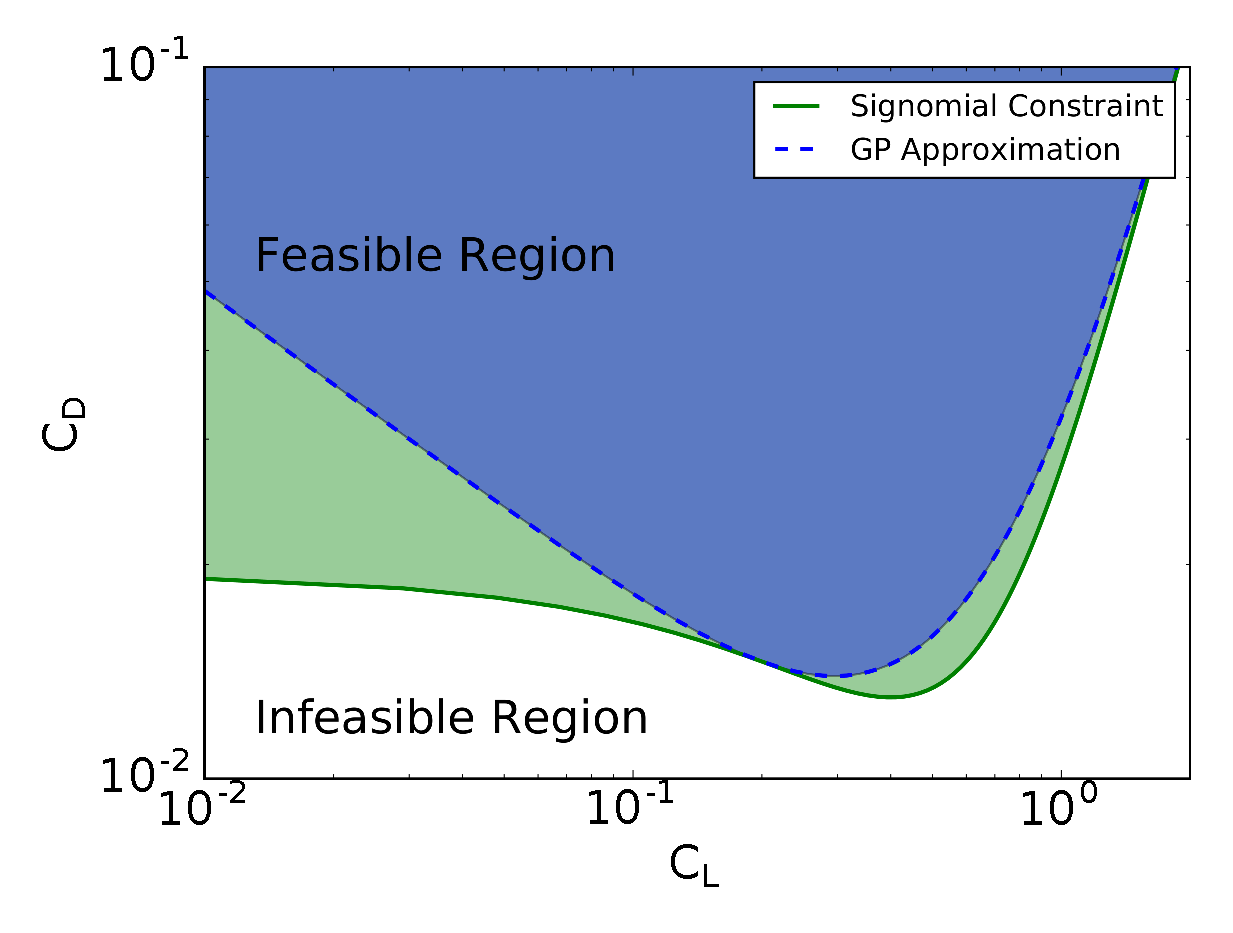
\includegraphics[width=0.9\linewidth]{posyapprox3.eps}
        \caption{Convex approximation about $C_{L} = 0.20.$}
    \end{subfigure}
    \caption{A signomial inequality constraint and GP approximations about two
different points.}
    \label{f:GPapproxs}
\end{figure*}

%\begin{figure}[htbp]
%\centering
%\subfloat[Non-convex signomial inequality drag constraint.]{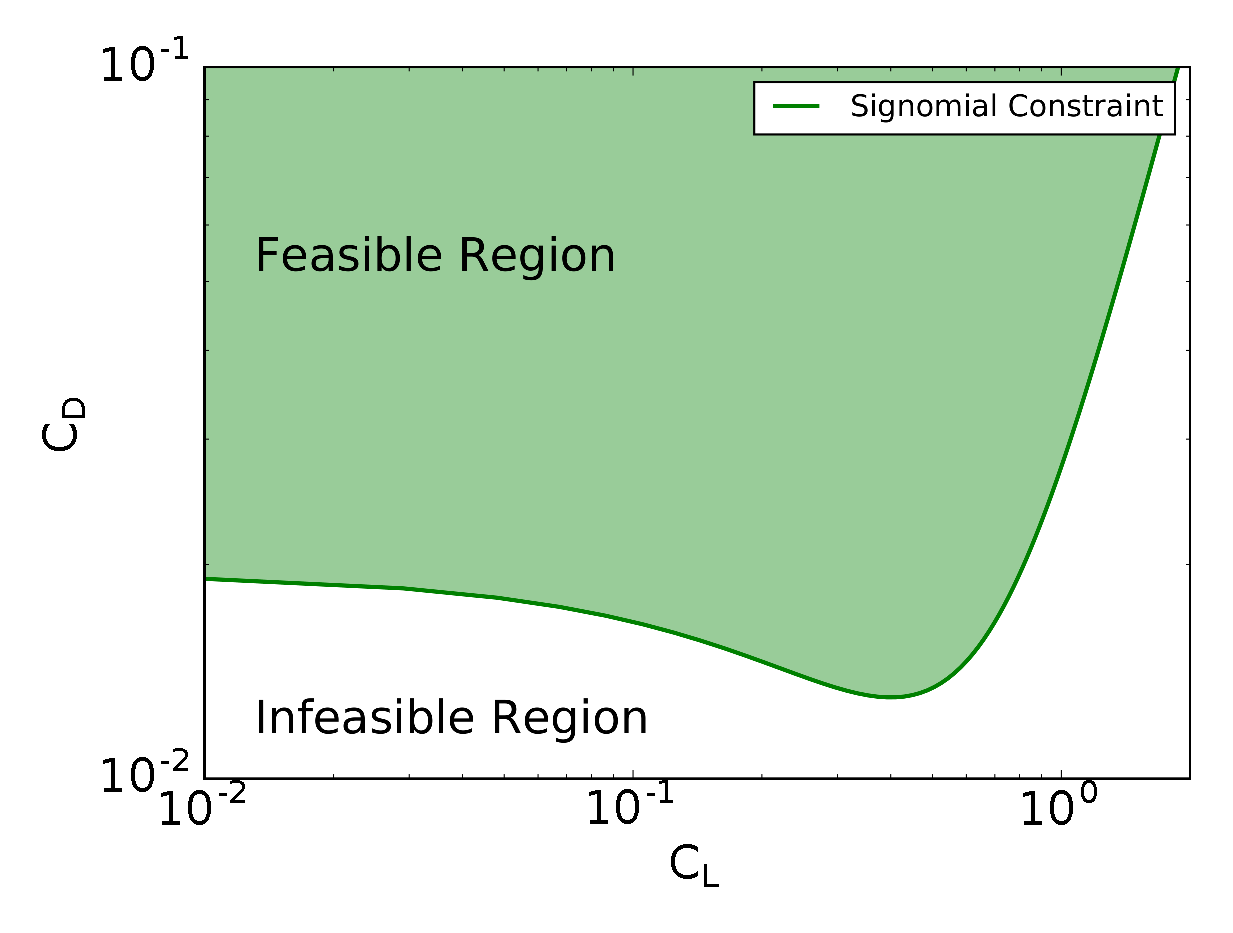
\includegraphics[width=0.45\textwidth]{posyapprox0.eps}}\hfill
%\subfloat[Convex approximation about $C_{L} = 0.05$.]{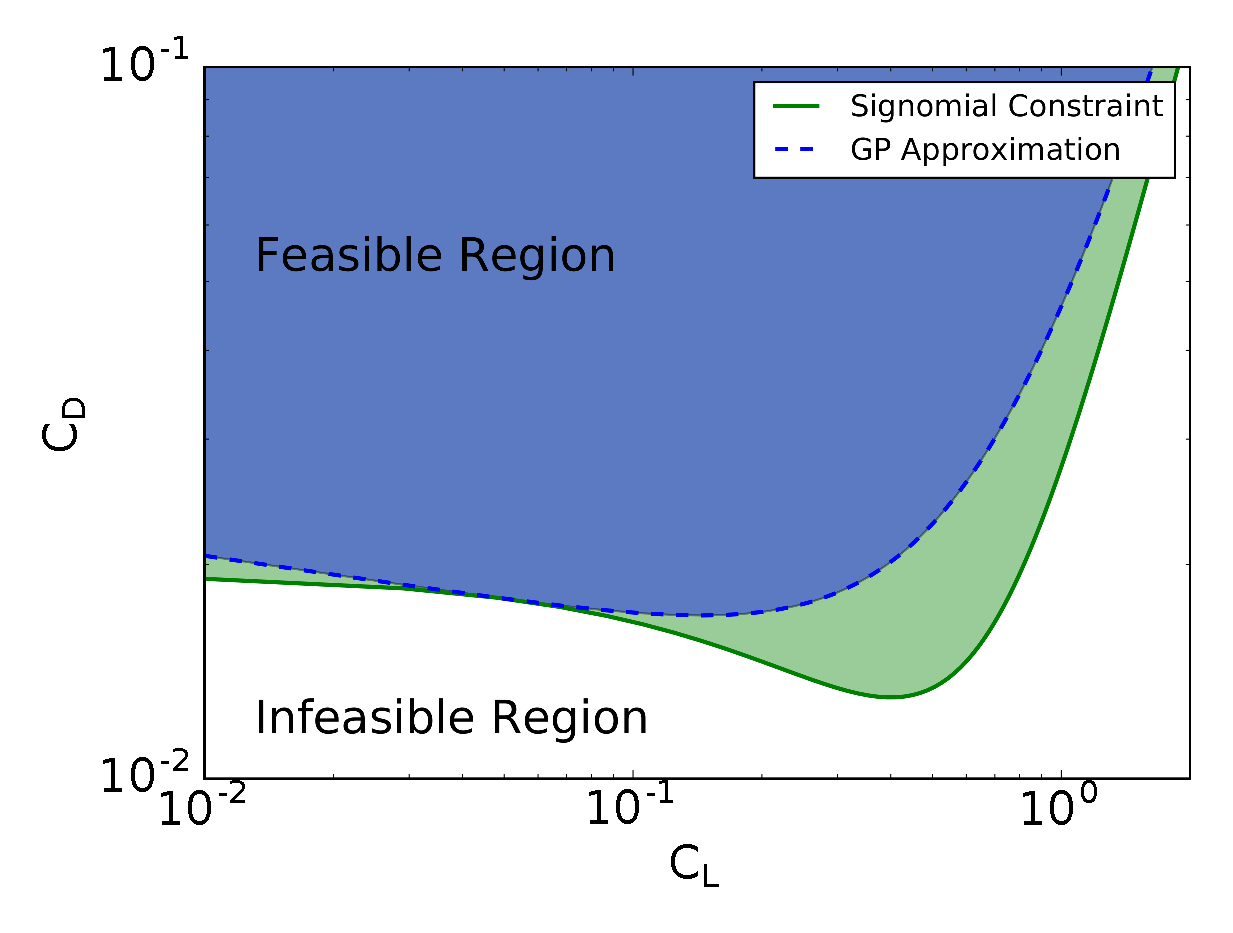
\includegraphics[width=0.45\textwidth]{posyapprox1.eps}}\hfill
%\subfloat[Convex approximation about $C_{L} = 0.20.$]{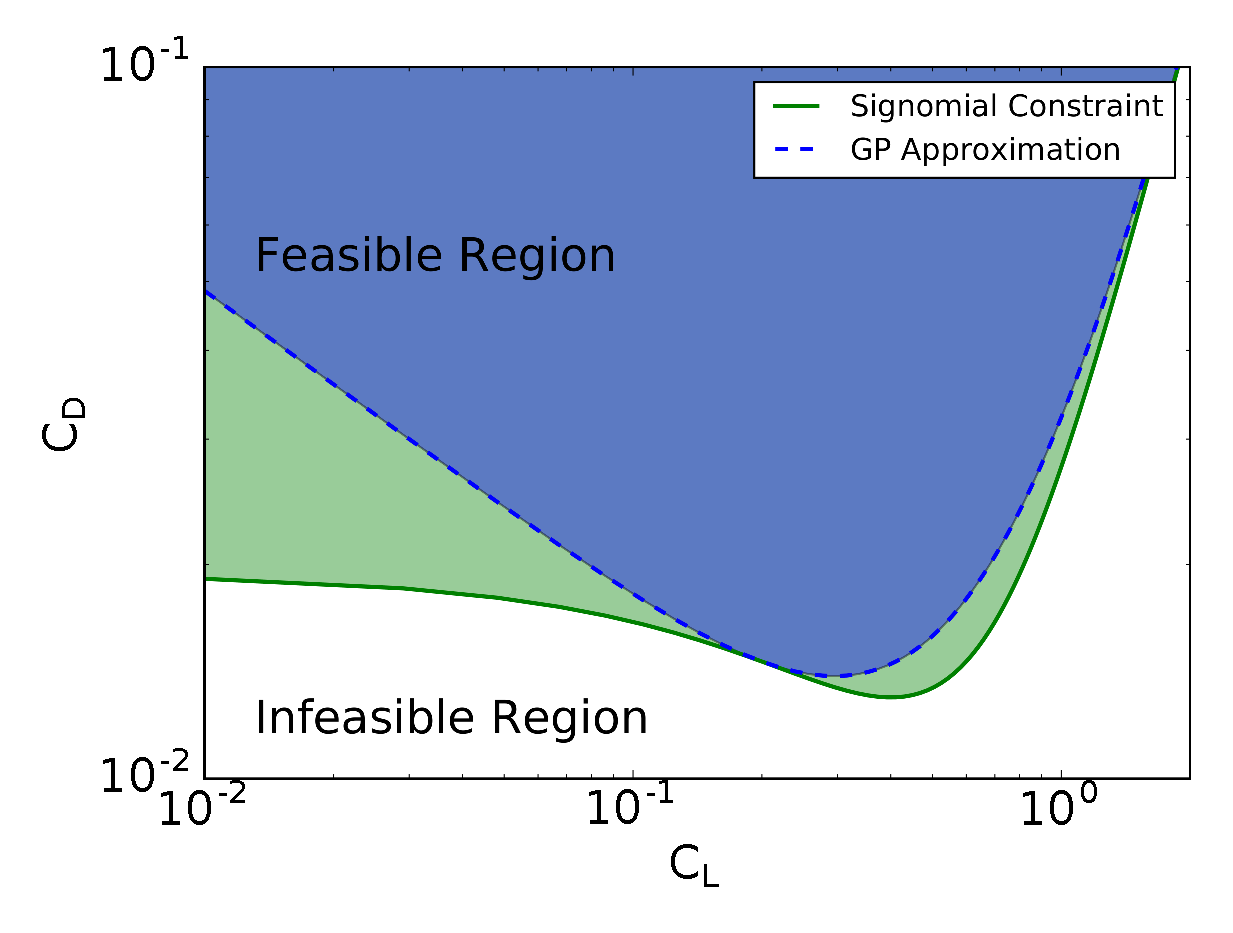
\includegraphics[width=0.45\textwidth]{posyapprox3.eps}}
%\caption{A signomial inequality constraint and GP approximations about two
%different points.} \label{f:GPapproxs}
%\end{figure}

Signomial equality constraints can be approximated by monomials as shown in
Figure~\ref{f:sigeq} and may require a trust region. Trust regions were not
used in the presented model. Signomial equalities are the least desirable type
of constraint due the approximations involved. Most constraints in this work
were relaxed to inequalities and checked for tightness by GPkit~\cite{gpkit}. For
additional details on how signomial equalities are approximated, see Opgenoord
et al.~\cite{sigeqpaper}.

\begin{figure}[!ht]
\centering
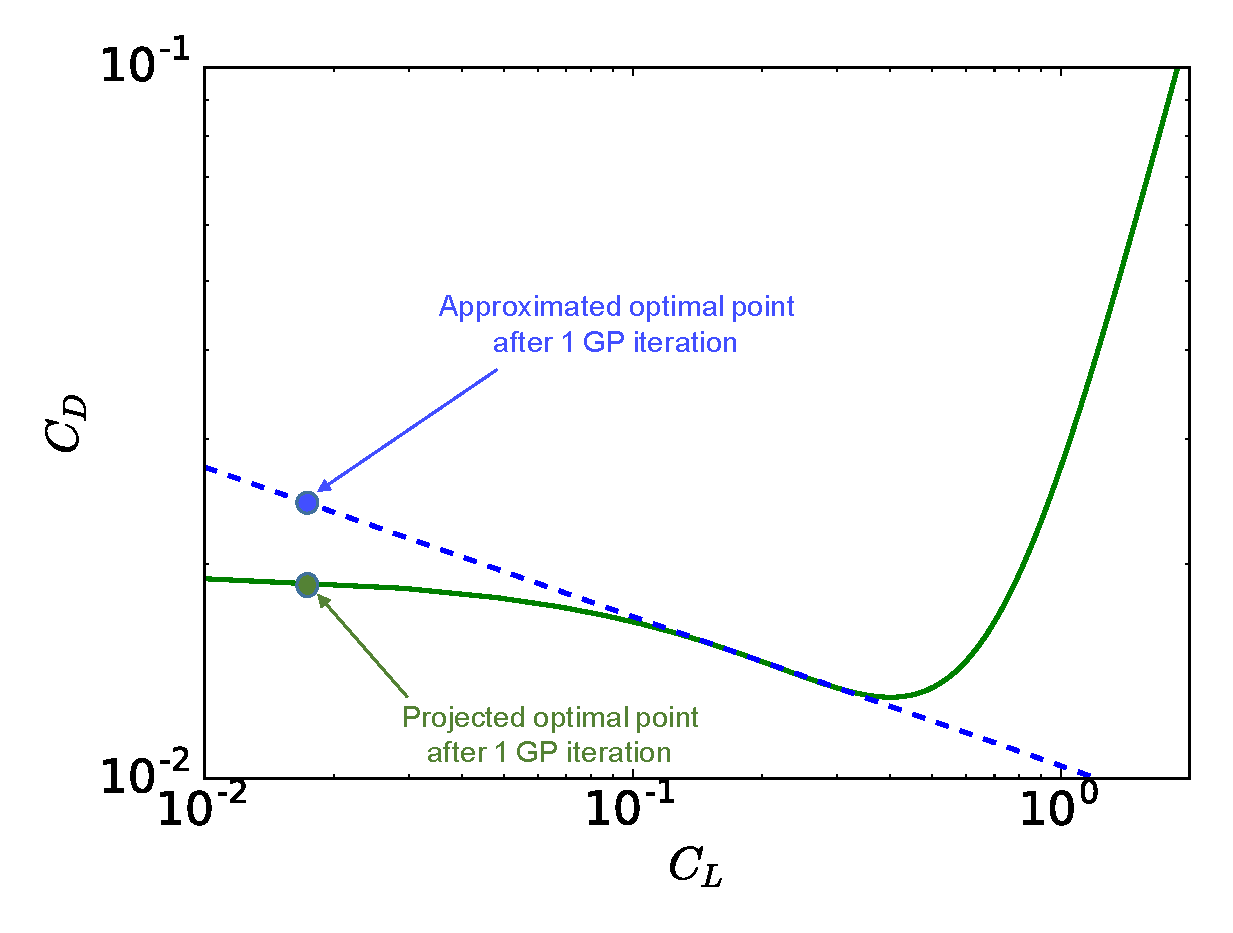
\includegraphics[width=0.45\linewidth]{sigeqapprox.eps}
\caption{The signomial equality constraint $C_{D} = f(C_{L})$ and its
approximation.}\label{f:sigeq}
\end{figure}

\section{Flight segment model variables}
\label{a:flightprofilevars}

\begin{footnotesize}
    \begin{table}
        \centering
        \begin{tabular}{l c l}
            \toprule
            Variable & Units & Description \\
            \midrule
            $\frac{dh}{dt}$  & $~\mathrm{\tfrac{m}{hr}}$ & climb rate \\
            $h$ & $~\mathrm{m}$ & segment flight altitude\\
            $h_{avg}$ & $~\mathrm{m}$ & segment flight altitude\\
            $R_s$ & $~\mathrm{km}$ & segment range\\
            $W_{start}$  & $~\mathrm{N}$ & segment beginning weight\\
            $W_{end}$ & $~\mathrm{N}$ & segment end weight\\
            $W_{avg}$ & $~\mathrm{N}$ & segment average weight\\
            $W_{f_s}$ & $~\mathrm{N}$ & segment fuel burn\\
            $W_{f_m}$  & $~\mathrm{N}$ & total mission fuel\\
            $t_s$ & $~\mathrm{hr}$ & segment time\\
            $t_m$  & $~\mathrm{hr}$ & total mission time\\
            \bottomrule
        \end{tabular}
        \caption{Variables introduced in flight segment model.}
        \label{t:vars_flightprofile}
    \end{table}
\end{footnotesize}
